\fenicschapter{An adaptive finite element solver for \\fluid--structure
               interaction problems}
              {An adaptive finite element solver for \\fluid--structure interaction problems}
              {Kristoffer Selim}
              {selim}
%% My commands
\definecolor{grey}{rgb}{0.5,0.5,0.5}
\newcommand{\subdt}{\textrm{d}_t}
\newcommand{\divv}{\textrm{div}\;}
\newcommand{\Divv}{\textrm{Div}\;}
\newcommand{\uF}{u_{_{F}}}
\newcommand{\dotuF}{\dot{u}_{_{F}}}
\newcommand{\pF}{p_{_{F}}}
\newcommand{\rhoF}{\rho_{_{F}}}
\newcommand{\sigmaF}{\sigma_{_{F}}}
\newcommand{\sigmaFup}{\sigma_{_{F}}(u_{_{F}}, p_{_{F}})}
\newcommand{\sigmaS}{\sigma_{_{S}}}
\newcommand{\bff}{b_{_{F}}}
\newcommand{\graduF}{\textrm{grad}\;u_{_{F}}}
\newcommand{\US}{U_{_{S}}}
\newcommand{\uS}{u_{_{S}}}
\newcommand{\GradUS}{\textrm{Grad}\;U_{_{S}}}
\newcommand{\ddotUS}{\ddot{U}_{_{S}}}
\newcommand{\ddotuS}{\ddot{u}_{_{S}}}
\newcommand{\PS}{P_{_{S}}}
\newcommand{\rhoS}{\rho_{_{S}}}
\newcommand{\SigmaS}{\Sigma_{_{S}}}
\newcommand{\SigmaSU}{\Sigma_{_{S}}(U_{_{S}})}
\newcommand{\BS}{B_{_{S}}}
\newcommand{\M}{\mathcal{M}}
\newcommand{\E}{\mathcal{E}}
\newcommand{\oF}{\omega_{_{F}}}
\newcommand{\oS}{\omega_{_{S}}}
\newcommand{\OS}{\Omega_{_{S}}}
\newcommand{\OF}{\Omega_{_{F}}}
\newcommand{\PhiS}{\Phi_{_{S}}}
\newcommand{\PhiM}{\Phi_{_{M}}}
\newcommand{\FS}{F_{_{S}}}
\newcommand{\UM}{U_{_{M}}}
\newcommand{\SigmaM}{\Sigma_{_{M}}}
\newcommand{\GradUM}{\textrm{Grad}\;U_{_{M}}}
\newcommand{\UF}{U_{_{F}}}
\newcommand{\PF}{P_{_{F}}}
\newcommand{\AFF}{A_{_{FF}}}
\newcommand{\AFS}{A_{_{FS}}}
\newcommand{\AFM}{A_{_{FM}}}
\newcommand{\ASS}{A_{_{SS}}}
\newcommand{\ASF}{A_{_{SF}}}
\newcommand{\ASM}{A_{_{SM}}}
\newcommand{\AMM}{A_{_{MM}}}
\newcommand{\AMF}{A_{_{MF}}}
\newcommand{\AMS}{A_{_{MS}}}

%------------------------------------------------------------------------------
Fluid--structure interaction (FSI) occurs when a fluid interacts with
a solid structure, exerting a stress that causes deformation of the
structure and, thus, alters the flow of the fluid itself. This vast
category of multiphysics problems are of great importance for
industrial related engineering applications, such as aircraft flutter,
and for the study of the human respiratory system, which is a
highly relevant research topic in biomedicine. The FSI problem is a
fully coupled multiphysics problem, whether the problem is solved in a
partitioned manner or by a monolithic approach. However, in
many cases we are only interested in one physical output quantity of
the fully coupled system, e.g., the displacement of the structure. In
order to compute this particular physical output of interest with a
high level of accuracy, a goal oriented adaptive finite element method
can be used.


This chapter gives a short introduction to goal oriented adaptive
finite element approximation for FSI problems and demonstrates how to
solve them using FEniCS. We start by formulating a FSI problem and
show how it is implemented in FEniCS, and then define and explain the
corresponding adaptive algorithm for the given FSI problem. For a more
comprehensive discussion on goal oriented adaptive finite element
methods for FSI problems, we refer to~\cite{SelimNarayananEtAl2010,
  Dunne2007, GratschBathe2006, BengzonLarson2010, Van2009,
  FickZeeBrummelen2008}.

%------------------------------------------------------------------------------
\section{Fluid--structure interaction}
\label{selim:sec:fsi}
Fluids and solids obey the fundamental conservation laws that hold
for any adiabatic continuum body: the balance of linear momentum and
the conservation mass.  These fundamental conservation laws can be
expressed in local form as
\begin{eqnarray}
\label{selim:eq:momentum}
\subdt(\rho u) - \Div \sigma &=& b, \\
\label{selim:eq:continuity}
\subdt(\rho )  &=& 0,
\end{eqnarray}
where~\eqref{selim:eq:momentum} is the balance of linear momentum
and~\eqref{selim:eq:continuity} is the conservation of mass.  Here,
$\subdt(\cdot)$ denotes the total time derivative, $\rho$ the density,
$u$ the velocity, $\sigma$ the stress, and $b$ represents a given body
force per unit volume. In a FSI problem, the different physical
quantities of the fluid and the structure, denoted with sub scripts
$F$ and $S$ respectively, transfer traction forces and exchange data
at a given common fluid--structure boundary.  Traction forces are
given by normal stresses and at the common fluid--structure boundary,
the following equilibrium equation holds:
\begin{equation}
\label{selim:eq:traction}
\sigma_{_{F}}\cdot n_{_{F}} = \sigma_{_{S}}\cdot n_{_{S}},
\end{equation}
where the fluid and structure normals are oriented such that
$n_{_{F}}= -n_{_{S}}$.  How a continuum responds to stress and in
particular to shear stress, distinguishes a fluid continuum from a
solid continuum. A fluid cannot withstand shear forces; it will
continue to deform as long as the stress is applied. Solids, on the
other hand, respond with an angular strain and the strain continues
until the displacement is sufficient to generate internal forces that
balance the imposed stress. To capture this, the constitutive laws
modeling fluids and solids relate the stress tensor to different
physical measures. Moreover, these measures are from a practical point
of view naturally posed in different frameworks, the so-called
Lagrangian framework and the Eulerian framework.

%------------------------------------------------------------------------------
\subsection{ Lagrangian framework and structure mechanics}

An essential kinematic measure in structure mechanics is the
displacement field which is naturally posed in the Lagrangian
framework.  In the Lagrangian framework, the motion of a body is
related to a fixed material point $x_0$ and the position of
such a point at time $t$ is given by the sufficiently smooth bijective
map $\phi$ that maps the point $x_0$ at time $t$ to the point $x(t)=
\phi(x_0,t)$. The \emph{structure displacement} is defined as
$\uS(x_0,t) = \phi(x_0, t) - x_0$ with the corresponding non-singular
Jacobi matrix $f = \Grad\phi$ and Jacobi determinant $j =
\textrm{det}\; f$. Thus, the total time derivative of a function $y$
in the Lagrangian framework is given by $\subdt(y) = \dot{y}$.
\\\\
Constitutive laws for hyperelastic materials express the stress
tensor $\sigma_{_{S}}$ (referred to as the first Piola--Kirchhoff
stress) as the Frech\'{e}t derivative of a given energy functional
$\psi$.  The energy functional can depend on different kinds of
kinematic measures, and if $\psi$ is dependent on the so-called
Green--Lagrange tensor $e= \tfrac{1}{2}(f^{\top}f -I)$, the corresponding first
Piola--Kirchhoff tensor is given by $\sigma_{_{S}} =
f\cdot\frac{\partial \psi(e)}{\partial e}$. In this chapter, we focus
on the compressible St. Venant--Kirchhoff model where the stress is
described by the energy functional $\psi(e) =
\mu_{_{S}}\textrm{tr}(e^2) +
\frac{\lambda_{_{S}}}{2}(\textrm{tr}(e))^2$, where
$(\mu_{_{S}},\lambda_{_{S}})$ are given positive Lam\'{e}
constants. Hence, the conservation laws for a ~St. Venant--Kirchhoff
material in the Lagrangian framework is given by
\begin{eqnarray}
\label{selim:eq:SVKmom}
\rhoS \ddotuS - \Div\sigmaS(\uS) &=& b_{_{S}}, \\
\label{selim:eq:SVKcon}
\dot{\rho}_{_{S}}&=&0,
\end{eqnarray}
with the corresponding stress tensor $\sigmaS(\uS) =
f\cdot(2\mu_{_{S}}e + \lambda_{_{S}} \textrm{tr}(e)I)$.  Note that we
usually omit the mass conservation equation~\eqref{selim:eq:SVKcon}
since it is automatically satisfied for compressible materials in the
Lagrangian framework.  For a more in depth analysis of hyperelastic
materials and structure mechanics in general, see~\cite{Gurtin1981,
  Holzapfel2000, Narayanan2007}.

%------------------------------------------------------------------------------
\subsection{Eulerian framework and fluid mechanics}
\label{selim:sec:fluid}
In fluid mechanics, the primary variables for describing the fluid
motion is the \emph{fluid velocity} $\uF$ and the \emph{fluid
  pressure} $\pF$. These variables are naturally posed in the Eulerian
framework where the motion of a body is related to a fixed spatial
point $x$ and the motion of the body is defined as $\uF(x,t) =
\uF(\phi(x_0,t),t)$. Thus, the total time derivative of a function $y$
in the Eulerian framework is given by $\subdt(y) = \dot{y} +
\textrm{grad}\;y\cdot\uF$.

The most common constitutive law for fluids is the Newtonian fluid
where the rate of strain is proportional to the rate of stress. For
Newtonian fluids, the stress tensor $\sigmaF$ (referred to as the
Cauchy stress) is given by $\sigmaFup = 2\mu_{_{F}}\varepsilon (\uF) -
\pF I$, where $\mu_{_{F}}$ denotes the dynamic viscosity and
$\varepsilon(\cdot)$ the symmetric gradient. In this chapter, we
assume that the fluid is an incompressible Newtonian fluid. The fluid
is then described by the classical incompressible Navier--Stokes
equations:
\begin{eqnarray}
  \label{selim:eq:NSmom}
      \rhoF(\dot{u}_{_{F}} + \textrm{grad}\;\uF\cdot\uF)- \divv
      \sigmaFup &=& b_{_{F}},\\
  \label{selim:eq:NScon}
      \divv \uF &=& 0.
\end{eqnarray}
For a more in depth analysis of constitutive laws for fluids and for
fluid mechanics in general, see~\cite{Batchelor1967,Panton1984,
  WeltyWicksWilson2001}.

%------------------------------------------------------------------------------
\section{FSI and the ALE computational framework}
\label{selim:sec:ale}
To combine the Lagrangian and the Eulerian frameworks in a
computational setting, the fluid traction force from
problem~\eqref{selim:eq:NSmom}-\eqref{selim:eq:NScon} is transferred
to the structure
problem~\eqref{selim:eq:SVKmom}-\eqref{selim:eq:SVKcon} via the Piola
map $(j\; (\sigma_{_{F}}\circ \phi)\cdot f^{-\top})\cdot n_{_{F}} =
\sigma_{_{S}}\cdot n_{_{S}}$ at the common fluid--structure boundary.
The deformation of the structure, given by the structure solution in
the material domain, needs to be tracked in the spatial fluid domain
and consequently, the mesh in the spatial fluid domain has to be
updated. A dynamically deforming mesh without any additional smoothing
algorithm to enhance the mesh quality will result in a mesh of poor
quality. To treat this shortcoming, an additional mesh equation is
posed in the fluid domain to enhance the mesh quality. Combining the
Lagrangian and the Eulerian frameworks with an additional mesh
smoothing algorithm is commonly referred to as the Arbitrary
Lagrangian--Eulerian (ALE) method, see~\cite{DoneaGiulianiHalleux1982,
  DoneaHuertaPonthotEtAl2004}.  In this method, both the Lagrangian
approach, in which the mesh of grid points moves with the structure,
and the Eulerian approach, in which the mesh represents a fixed
reference frame for the fluid, are used. In order to incorporate the
mesh equation in the FSI problem, an arbitrary reference frame for the
fluid domain is introduced which is independent of the Lagrangian
description and the Eulerian description. This arbitrary reference
domain is typically the initial undeformed computational domain.

Let $\Omega$ be a fixed open domain in $\mathbb{R}^d$ which represents
the \emph{reference} (undeformed) computational domain, for
$d=2,3$. Moreover, let $\Omega$ be partitioned into two disjoint open
subsets $\OF$ and $\OS$ such that
$\bar{\Omega}_{_{F}}\cup\bar{\Omega}_{_{S}} = \Omega$ and
$\OF\cap\OS=\emptyset$. Further, let $\omega(t)\in\mathbb{R}^d$ denote
the \emph{current} (deformed) computational domain which is similarly
partitioned into two disjoint subsets $\oF(t)$ and $\oS(t)$ such that
$\bar{\omega}_{_{F}}\cup\bar{\omega}_{_{S}} = \omega$ and
$\oF(t)\cap\oS(t)=\emptyset$, for all time $t\in[0,T]$. The common
boundary between the structure and fluid domains is denoted by
$\Gamma_{FS}$ and $\gamma_{FS}(t)$ respectively. To distinguish
between variables and operators associated with the reference and
current domains, we use upper case and lower case letters
respectively. Thus, $\Divv\SigmaS(\US(X,t))$ is the divergence of the
structure stress defined on the reference structure domain $\OS$, and
$\graduF(x,t)$ is the current gradient of the fluid velocity defined
in the current fluid domain $\oF(t)$.

In order to map between the reference domain and the current domain,
we introduce the sufficiently smooth bijective map $\Phi(\cdot,
t):\Omega\mapsto \omega(t)$.  For any fixed time $t\in[0,T]$, $\Phi$
maps a reference point $X\in\Omega$ to the corresponding current
point $x\in\omega(t)$, i.e., $X \mapsto x = \Phi(X,t)$.
\begin{figure}
  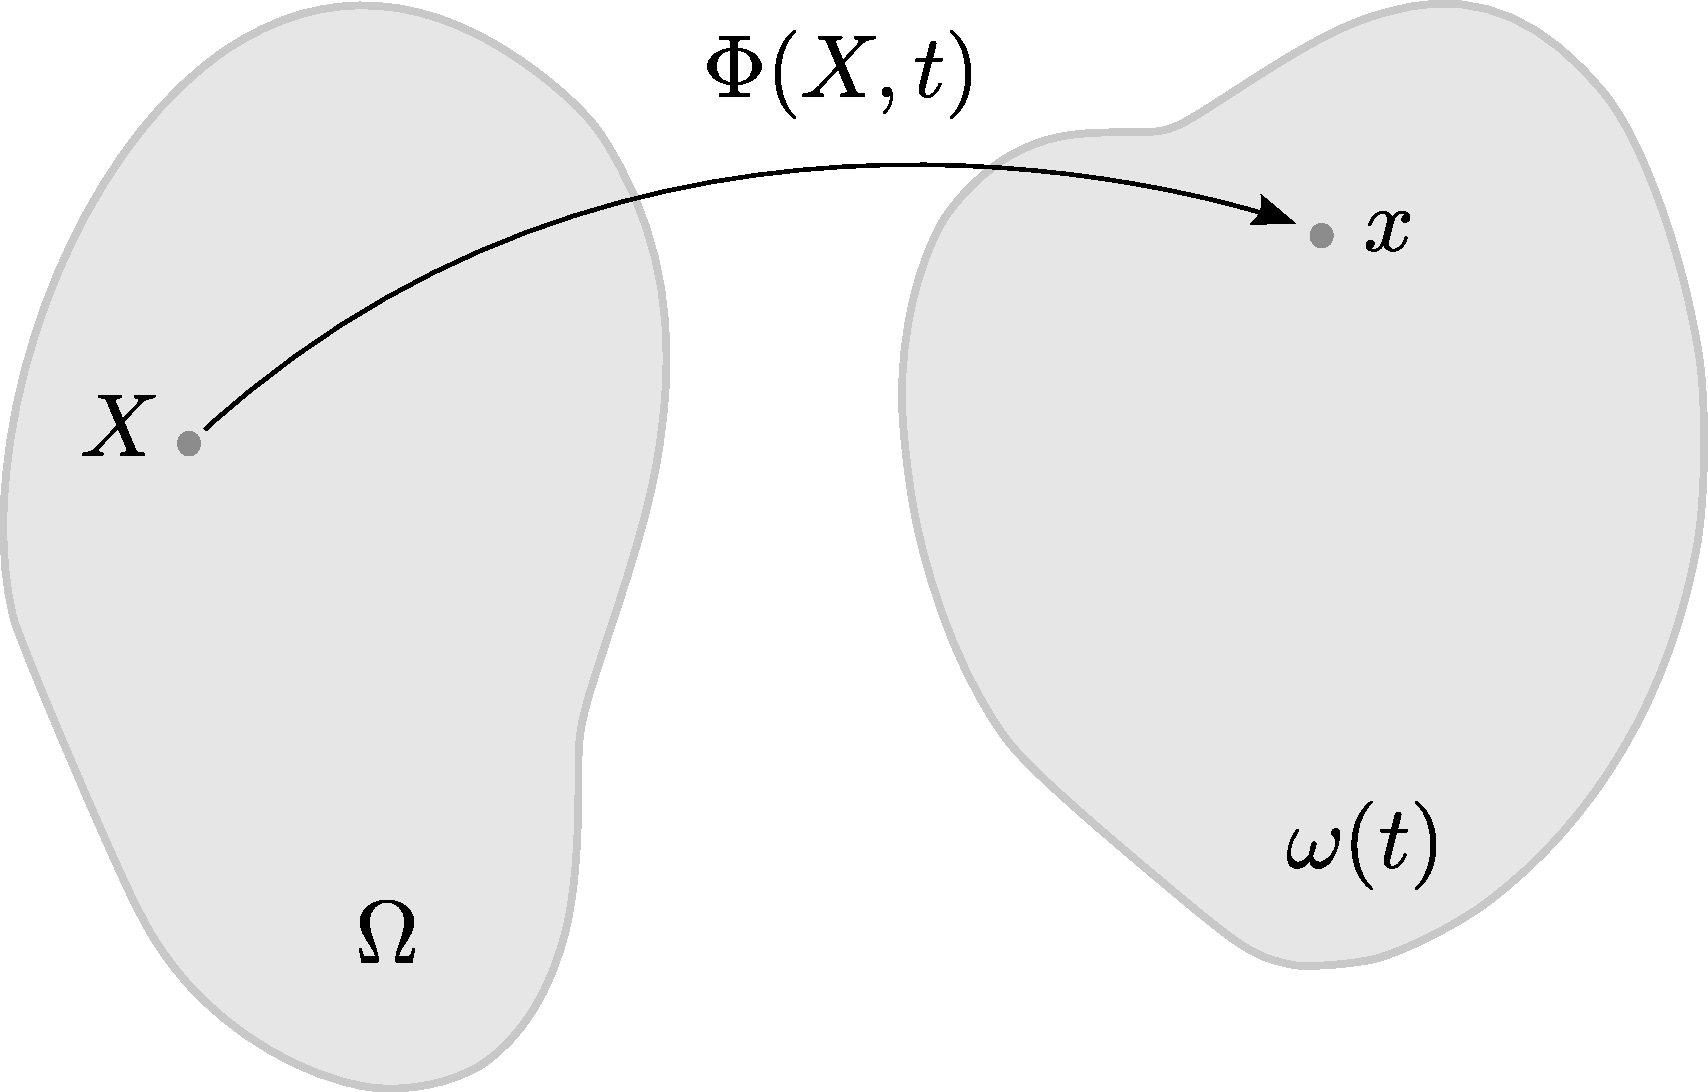
\includegraphics[width=0.8\textwidth]{chapters/selim/pdf/mapping.pdf}
 \caption{The mapping $\Phi(X,t$) maps a reference point $X\in\Omega$
   to the current point $x\in\omega(t)$. The deformation gradient of
   the reference domain $\Omega$ is given by $\textrm{Grad}\:\Phi =
   F$, and the volume change of $\Omega$ is thus $J = \textrm{det}(F)$.}
 \label{selim:fig:mapping}
\end{figure}
\\
Since we allow the fluid and structure portions of the domain to
deform independently (only enforcing that these deformations are
identical on the common boundary), the map is split up as follows:
\begin{equation}
\label{selim:eq:ALEmapI}
\Phi(X,t) =
\left\{
\begin{array}{ccc}
\PhiS(X, t), \quad \forall X\in\OS,\; t\in[0,T],\\
\PhiM(X, t), \quad \forall X\in\OF,\; t\in[0,T].
\end{array}
\right.
\end{equation}
Here, the structure map and the (fluid) mesh map $(\PhiS, \PhiM)$ are
defined as
\begin{eqnarray}
\label{selim:eq:ALEmapII}
\PhiS(X, t) &=& X + \US(X,t),\\
\PhiM(X, t) &=& X + \UM(X,t),
\end{eqnarray}
where $(\US, \UM)$ are the solutions to the structure problem and the
arbitrarily chosen mesh problem, respectively.  There are several
possibles ways to formulate and solve the mesh problem to obtain
$\UM$, see~\cite{HermanssonHansbo2003, LopezNigroStorti2008}.  In the
following, we have adopted a time dependent mesh problem related to a
linear elastic description of the fluid domain in which the stress
tensor is given by $\SigmaM(\UM)\equiv \mu_{{_M}}(\GradUM +
\GradUM^{\top})+ \lambda_{_{M}}\textrm{tr}(\GradUM)I$ for some given
positive constants $(\mu_{{_M}},\lambda_{_{M}})$.

To summarize, we identify the three subproblems that together define
the fully coupled FSI problem:
\begin{itemize}
\item
the fluid problem $(f)$ solved in the current fluid domain $\oF(t)$;
\item
the structure problem $(S)$ solved in the reference structure domain;
$\OS$
\item
the mesh problem $(M)$ solved in the reference fluid domain $\OF$.
\end{itemize}
The corresponding set of equations for the triplet
$(f),(S),(M)$ is given by:
\begin{equation}
  \addtolength{\fboxsep}{5pt} \boxed{
    \begin{split}\label{selim:eq:FSIsystem}
   &(f):&\quad \rhoF(\dotuF + \graduF\cdot\uF) -
      \divv\sigmaF(\uF,\pF) =\;& \bff \quad
      \textrm{in}\;\oF(t)\\ &&\divv\uF =\;&
      0\:\:\quad\textrm{in}\;\oF(t) \\\\ &(S):&\quad \rhoS \ddotUS -
      \Divv \SigmaS(\US) =\;& \BS \quad \textrm{in}\; \OS\times
      (0,T]\\\\ &(M):&\quad \dot{U}_{_{M}} - \Divv \SigmaM(\UM) =\;& 0
  \;\:\quad\textrm{in}\; \OF\times (0,T]
    \end{split}
  }
\end{equation}
together with initial and boundary conditions. We note that, with the
proposed notation, the stress from the fluid is transferred to the
structure and the movement of the structure is tracked in the fluid
domain at the common fluid--structure boundary such that:
\begin{equation}
  \addtolength{\fboxsep}{5pt} \boxed{
    \begin{split}\label{selim:eq:ALEtraction}
      (J_{_{M}}\;(\sigmaF\circ\PhiM) \cdot F_{_{M}}^{-\top})\cdot
      N_{_{F}} &= \SigmaS\cdot N_{_{S}} \quad &\textrm{on}\; \Gamma_{FS}\\
      \uF\circ\PhiM &= \dot{\Phi}_{_{S}} \quad &\textrm{on}\; \Gamma_{FS}\\
    \end{split}
  }
\end{equation}
Thus, \eqref{selim:eq:ALEtraction} transfers data between all the
equations in the FSI system~\eqref{selim:eq:FSIsystem} at the common
FSI interface.

In the numerical solution of the fluid problem $(f)$,
we compensate for the additional mesh movement $\dot{u}_{_{M}}$ in the
fluid domain $\oF(t)$ introduced by the mesh equation $(M)$.  The
resulting discrete finite element form of the convective term of the
fluid problem takes the form $\rhoF(\dotuF^{hk} +
\graduF\cdot(\uF^{hk} - \dot{u}_{_{M}}^{hk}))$.  This additional mesh
movement is a pure numerical artifact and is not a part of the
continuum representation of the FSI problem.

%------------------------------------------------------------------------------
\section{The FSI solver}
\label{selim:sec:primalsolver}
The proposed system of equations that defines the fully coupled FSI
problem~\eqref{selim:eq:FSIsystem} is a partitioned system, where the
subproblems $(f),(S),(M)$ are connected at the fluid--structure
interface with the boundary conditions
in~\eqref{selim:eq:ALEtraction}. To solve such a system, the
subproblems are iteratively solved using the following simple fixed
point algorithm:
\begin{enumerate}
\item
Solve the fluid problem $(f)$
\item
Transfer the fluid stress using~\eqref{selim:eq:ALEtraction} and
solve the structure problem $(S)$
\item
Solve the mesh problem $(M)$ and update the fluid domain
\item
Repeat steps (1) -- (3) until convergence
\item
Move on to the next time step
\end{enumerate}
\begin{figure}
  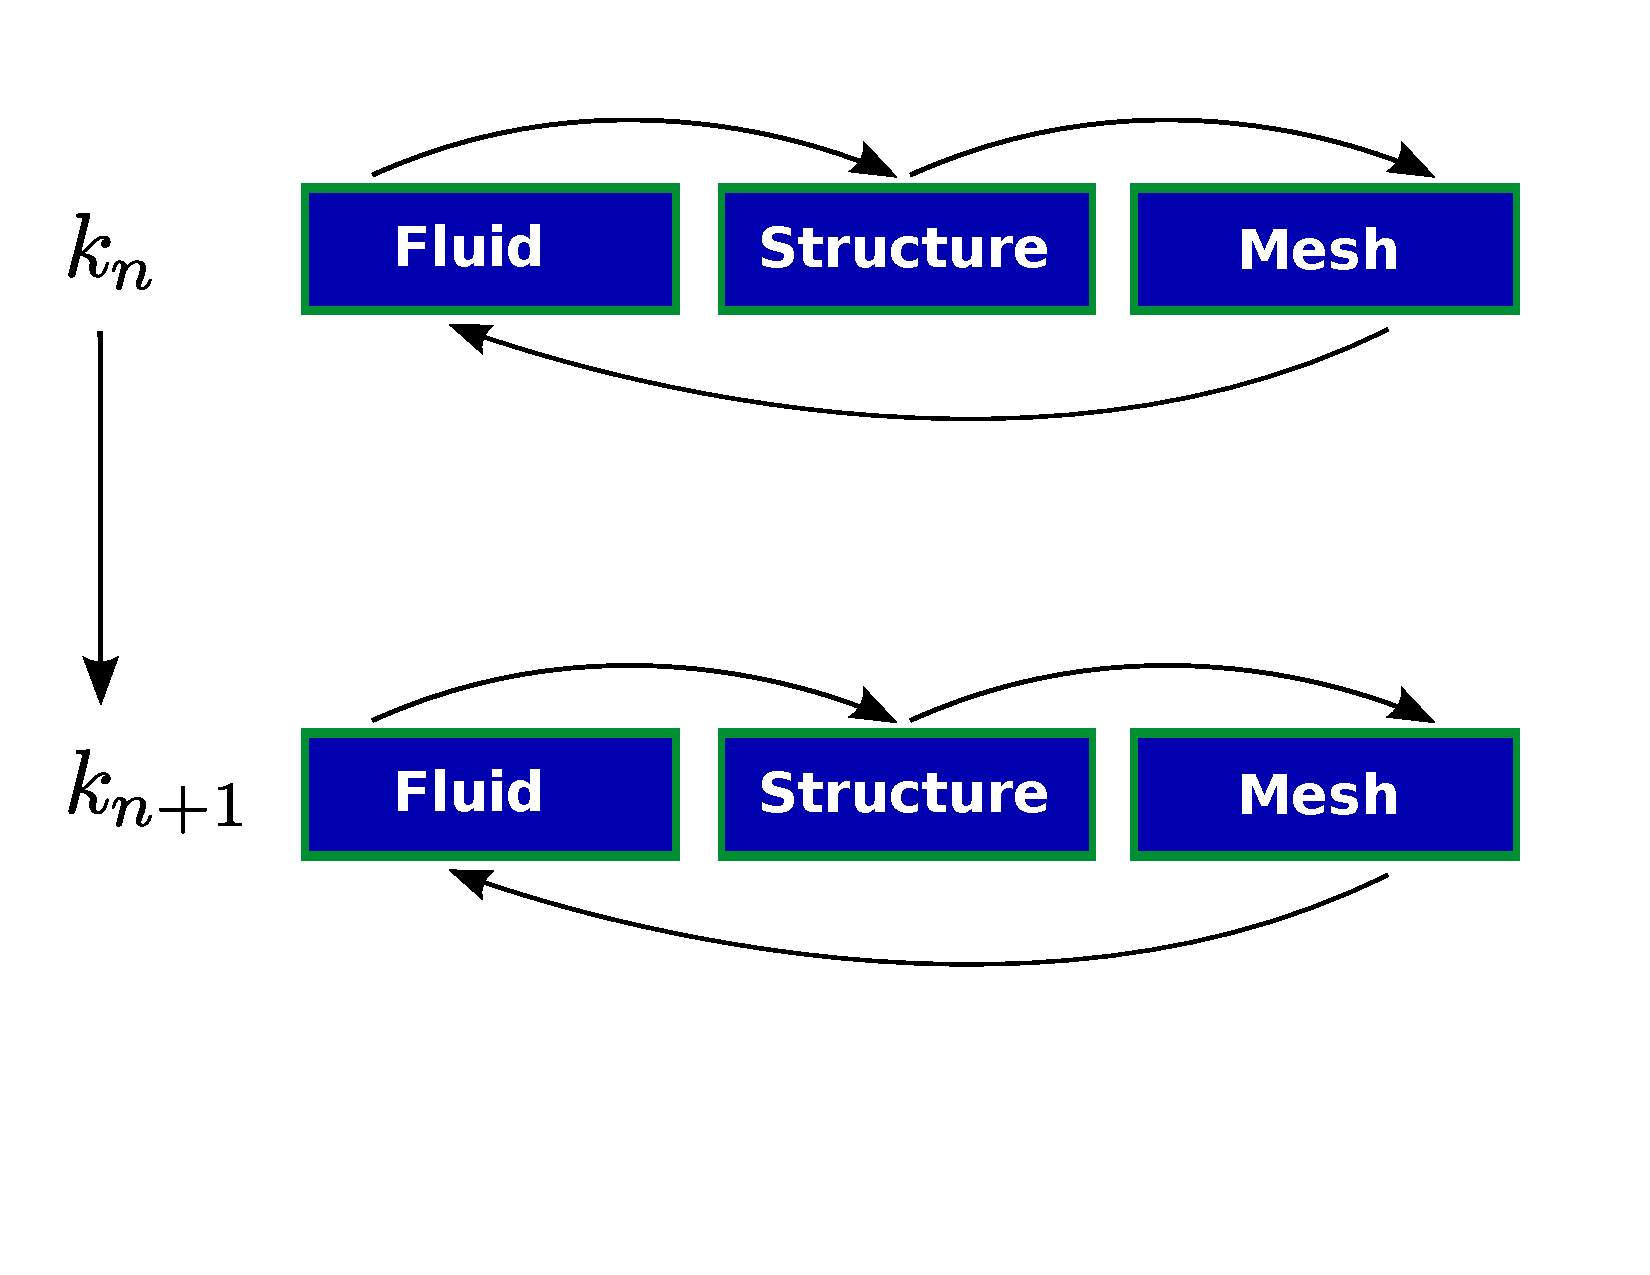
\includegraphics[width=0.85\textwidth]{chapters/selim/pdf/primal.pdf}
  \caption{A partitioned approach to solving the FSI problem. In each
    time step $k_n$, the three subproblems are solved iteratively
    using a simple fixed point method. The fluid problem is first
    solved on the given current fluid domain $\oF(t)$ and the stress
    $\sigmaF$ is evaluated and transferred (mapped back) to the
    structure problem in the reference domain. In the structure
    reference domain $\Omega_{_{S}}$, the fluid stress is set as a
    Neumann condition and the structure problem is solved for the
    given fluid stress. The structure displacement field is then set
    as a Dirichlet boundary condition at the common fluid--structure
    boundary for the mesh equation in the fluid reference domain
    $\Omega_{_{F}}$. Having obtained the mesh solution, the solution
    is pushed forward to the current fluid domain and thus defines the
    new deformed current domain.}
\end{figure}
The two subproblems $(f)$, $(S)$ in~\eqref{selim:eq:FSIsystem} define
a classic set of equations from fluid mechanics and structure
mechanics. To solve the coupled system, a solver framework for
handling both types of physics is needed. For this purpose, we have
used the multiphysics framework \texttt{CBC.Solve} developed at the
Center for Biomedical Computing at Simula Research Laboratories in
Oslo. Currently, \texttt{CBC.Solve} consists two core components;
\texttt{CBC.Flow} and \texttt{CBC.Twist} which are frameworks
explicitly developed for solving fluid mechanics problems and
structure mechanics problems, respectively.  In the subsequent
sections, we will briefly explain these frameworks and the code that
solves the FSI problem~\eqref{selim:eq:FSIsystem}.

%------------------------------------------------------------------------------
\subsection{Fluid subproblem}

The fluid subproblem in~\eqref{selim:eq:FSIsystem} is solved using the
\texttt{CBC.Solve} module \texttt{CBC.Flow}. Currently, the solver
handles incompressible Newtonian fluids only, but its overall goal is
to implement a solver that can solve a larger class of fluid problems.
The fluid problem can be solved in an Eulerian coordinate system or in
an ALE coordinate system, and the solver is based on the stress
formulation of the so-called Incremental Pressure Correction Scheme
(IPCS)~\cite{Goda1979}. The fluid velocity $\uF$ and the fluid
pressure $\pF$ are discretized in space using Taylor--Hood
elements. The resulting nonlinear variational problem is solved in
three steps. In the first step, the tentative fluid velocity is
computed from the momentum equation using the previously known
pressure. After this step, the pressure at the current time step is
computed and corrected using the continuity equation. Finally, in the
third step, the velocity is corrected using the corrected pressure.
The implementation is illustrated with a code segment from the class
\texttt{NavierStokesSolver} in Figure~\ref{selim:fig:fluidsolver}. For
a more comprehensive discussion how to solve and implement different
solvers for the incompressible Navier--Stokes equations in FEniCS, see
Chapter~\ref{chap:kvs-1}.
\begin{figure}
\begin{center}
\begin{python}
 class NavierStokesSolver(CBCSolver):
    "Navier-Stokes solver"

   def __init__(self, problem):
        "Initialize Navier-Stokes solver"

        ...

        # Tentative velocity step (sigma formulation)
        U = 0.5*(u0 + u)
        F1 = rho*(1/k)*inner(u - u0, v)*dx \
           + rho*inner(grad(u0)*(u0 - w), v)*dx \
           + inner(sigma(U, p0), epsilon(v))*dx \
           + inner(p0*n, v)*ds \
           - mu*inner(grad(U).T*n, v)*ds \
           - inner(f, v)*dx
        a1 = lhs(F1)
        L1 = rhs(F1)

        # Pressure correction
        a2 = inner(k*grad(p), grad(q))*dx
        L2 = inner(k*grad(p0), grad(q))*dx \
           - div(u1)*q*dx

        # Velocity correction
        a3 = inner(u, v)*dx
        L3 = inner(u1, v)*dx \
           + inner(k*grad(p0 - p1), v)*dx
\end{python}
\caption{A code segment of the fluid solver in \texttt{CBC.flow}. The
  momentum equation is multiplied with a test function \texttt{v} and
  the continuity equation is multiplied with a test function
  \texttt{q}. In the first step, the tentative velocity is computed
  from the momentum equation using a fully implicit formulation of the
  convective term and the previously computed pressure. Here, \texttt{w}
  denotes the mesh velocity $\dot{u}_{_{M}}$. In the next step, the
  pressure is corrected with the continuity equation based on the
  computed velocity \texttt{u1} from the first step. Finally, the
  velocity is corrected using the corrected pressure.}
\label{selim:fig:fluidsolver}
\end{center}
\end{figure}

%------------------------------------------------------------------------------

\subsection{Structure subproblem}

\texttt{CBC.Twist} is a solver collection for structure mechanics
problems. This module solves the given structure problem in a
Lagrangian coordinate system.  The solver allows the user to easily
pose problems and provides many standard material models, including
St.~Venant--Kirchhoff, Mooney--Rivlin, neo--Hookean, Isihara, Biderman
and Gent--Thomas. New models may be added easily since the interface
allows the user to provide an energy functional as function of a
suitable kinematic measure, such as the Green--Lagrange strain. Both a
static and an energy-momentum preserving time-dependent solver are
provided. The space discretization relies upon first order Lagrange
elements and for the time discretization several different schemes are
available, such as the $cG(1)$
method~\cite{ErikssonEstepHansboEtAl1996, ErikssonEstepJohnson2003} or
the "HHT'' method~\cite{HilberHughesTaylor1977}.  In the $cG(1)$
method, used in this chapter, the structure problem is re-written as a
first order system in time by introducing the additional equation
$P_{_{S}} - \dot{U}_{_{S}} = 0$ to the structure equation $(S)$
in~\eqref{selim:eq:FSIsystem}. The structure stress tensor, regardless
of material model, is given as the first Piola--Kirchhoff tensor and
the nonlinear variational problem is solved using Newton's method.
The implementation of the $cG(1)$ version is illustrated in the code
segment from the class \texttt{CG1MomentumBalanceSolver} in
Figure~\ref{selim:fig:structuresolver}. For a more comprehensive
discussion of how to solve structure problems using
\texttt{CBC.Twist}, and especially how to implement different material
models, see Chapter~\ref{chap:narayanan}.

\begin{figure}
\label{selim:fig:structuresolver}
\caption{A code segment from the $cG(1)$ version of the structure
  solver \texttt{CBC.Twist}.  The momentum equation is multiplied with
  test functions \texttt{v}, \texttt{q} and adding the two equations
  yields the nonlinear variational form \texttt{L}. The nonlinear
  variational form \texttt{L} contains the structure velocity
  \texttt{p} and the first Piola--Kirchhoff stress tensor
  \texttt{sigma} (which is a function of the structure
  displacement $\US$).  The nonlinear form \texttt{L} is
  linearized using the FEniCS function \texttt{derivative} where
  \texttt{U} represents the mixed finite element space containing the
  structure solution $(\US, P_{_{S}})$.  We note that Neumann
  conditions, such a fluid stress, are imposed in the variational form
  \texttt{L} while the Dirichlet conditions are set directly in the
  Newton solver. We also note that the proposed variational form holds
  for a vast amount of different structure models, where the first
  Piola--Kirchhoff stress tensor \texttt{sigma} is given by an
  appropriate material model.  }
\begin{python}
class CG1MomentumBalanceSolver(CBCSolver):
    """Solves the dynamic balance of linear momentum using a CG1
    time-stepping scheme"""

    def __init__(self, problem):
        """Initialize the momentum balance solver"""

        ...

        # The variational form corresponding to hyperelasticity
        L = rho0*inner(p - p0, v)*dx + k*inner(sigma, grad(v))*dx \
          - k*inner(b, v)*dx + inner(u - u0, q)*dx \
          - k*inner(p_mid, q)*dx

        # Add contributions to the form from the Neumann boundary
        # conditions
        neumann_conditions = problem.neumann_conditions()
        neumann_boundaries = problem.neumann_boundaries()

        boundary = MeshFunction("uint", mesh, mesh.topology().dim() - 1)
        boundary.set_all(len(neumann_boundaries) + 1)

        for (i, neumann_boundary) in enumerate(neumann_boundaries):
            compiled_boundary = compile_subdomains(neumann_boundary)
            compiled_boundary.mark(boundary, i)
            L = L - k*inner(v, neumann_conditions[i])*ds(i)

        a = derivative(L, U, dU)
\end{python}
\end{figure}

\newpage
%------------------------------------------------------------------------------
\subsection{Mesh subproblem}

The linear mesh subproblem is solved using first order Lagrange
elements in space along with a standard $cG(1)$ formulation in time.
The implementation of the mesh subproblem is illustrated in
Figure~\ref{selim:fig:meshsolver}.
\begin{figure}
\caption{A code segment of the mesh solver \texttt{MeshSolver}.}
\label{selim:fig:meshsolver}
\begin{python}
  # Define cG(1) scheme for time-stepping
  a = inner(u, v)*dx + 0.5*k*inner(sigma(u), sym(grad(v)))*dx
  L = inner(u0, v)*dx - 0.5*k*inner(sigma(u0), sym(grad(v)))*dx
\end{python}
\end{figure}

%------------------------------------------------------------------------------
\section{Duality--based error control}

As mentioned in the beginning of this chapter, in many cases we are
only interested in computing one output quantity of the fully coupled
FSI system. This output quantity is commonly referred to as the goal
functional.  To assure a high level of accuracy of the functional of
interest, the error in the goal functional needs to be controlled. In
finite element discretizations, classic a posteriori error analysis
provides a general framework for controlling the approximation error
of the solution.  The extension of the classical a posteriori error
analysis to controlling the error of a goal functional has been under
development over the past two decades, and the technique originates
form ~\cite{ErikssonEstepHansboEtAl1995, BeckerRannacher2001}. This
technique is based on the solution of an auxiliary linearized dual
(adjoint) problem in order to estimate the error in a given goal
functional. By solving the dual problem, one may construct an adaptive
algorithm that targets efficiently the computation of a specific goal
functional $\M$ of interest, such that
\begin{equation}
  \label{selim:eq:goalTOL}
|\M(U)-\M(U^{hk})| \leq \mathrm{TOL}.
\end{equation}
Here, $ U-U^{hk} \equiv e$ is the error of the finite element solution
in space $(h)$ and time $(k)$, and $\mathrm{TOL}>0$ is a user-defined
tolerance.  To define the dual problem for the FSI
problem~\eqref{selim:eq:FSIsystem}, we pull back the fluid subproblem
$(f)$ from the current fluid domain $\oF(t)$ to the fluid reference
domain $\OF$ using the map $\PhiM$,
\begin{equation}
  \label{selim:eq:pullback}
  \begin{CD}
    (F) @<\PhiM^{-1}<< (f).
  \end{CD}
\end{equation}
With the fluid problem $(F)$ defined in the reference domain, all the
three sub problems $(F,S,M)$ are posed in the reference domain
$\Omega$, and we may thus formulate a monolithic counterpart to the
FSI problem~\eqref{selim:eq:FSIsystem}. The abstract nonlinear
variational form reads: Find $U\equiv \{ \UF, \PF, \US, \PS, \UM,
P_{_{M}} \}\in V$ such that
\begin{equation}
\label{selim:eq:monolithic}
a(U;v) = L(v),
\end{equation}
for all $v\equiv \{ v_{_{F}}, q_{_{F}}, v_{_{S}}, q_{_{S}}, v_{_{M}}, q_{_{M}}
\}\in\hat{V}$, where the trial and test spaces $(V,\hat{V})$ are
associated with the geometrically conforming parts of $\Omega_{_{F}}$
and $\Omega_{_{S}}$, respectively. By introducing the linearized
variational form $a'(U; \delta U,v ) \equiv \frac{\partial
  a(U;v)}{\partial U}\delta U$, we note that by the chain rule
\begin{eqnarray}
\overline{a}(e, v) \equiv \overline{a}(U,U^{hk};e, v) &\equiv& \int_0^1 a'(sU + (1-s)U^{hk}; e,
v) \ds \\ &=& \int_0^1 \frac{\textrm{d}}{\ds} a (sU + (1-s)U^{hk}; v)
\ds \\ &=& L(v) - a(U^{hk};v) \\ &\equiv&  r(v),
\end{eqnarray}
where $r(\cdot)$ is the (weak) residual of~\eqref{selim:eq:monolithic}.
We now define the following dual problem: Find the dual solution
$Z\equiv \{ Z_{_{F}}, Y_{_{F}}, Z_{_{S}}, Y_{_{S}}, Z_{_{M}},
Y_{_{M}}\}\in V^*$ such that
\begin{equation}
  \label{selim:eq:dual}
  \overline{a}^{*}(Z, v) = \M(v),
\end{equation}
for all $v\equiv \{ v_{_{F}}, q_{_{F}}, v_{_{S}}, q_{_{S}}, v_{_{M}}, q_{_{M}}
\}\in\hat{V}^*$.

We may express the dual problem on block form as
\begin{eqnarray}
\label{selim:eq:dualsystem}
\left[\begin{array}{ccc} \hat{v}_{_{F}} & \hat{v}_{_{S}} & \hat{v}_{_{M}}
  \end{array} \right]
\left[\begin{array}{lll} \AFF & \textcolor{grey}{\AFS} & \AFM
    \\ \ASF & \ASS & \ASM \\ \textcolor{grey}{\AMF} & \AMS &
    \AMM
\end{array} \right]^{\top}
\left[ \begin{array}{c} \hat{Z}_{_{F}} \\ \hat{Z}_{_{S}}
    \\ \hat{Z}_{_{M}} \end{array} \right] =\left[ \begin{array}{l}
    \M_{_{F}}\\ \M_{{_S}}\\ \M_{_{M}} \end{array} \right].
\end{eqnarray}
Here, $\hat{v}_{_{F}} = (v_{_{F}}, q_{_{F}})$ represents the fluid
test functions, $\AFF$ denotes the fluid problem linearized around the
fluid variables $(\UF,\PF)$, $\hat{Z}_{_{F}} = (Z_{_{F}}, Y_{_{F}})$
are the dual fluid variables and $\M_{_{F}}$ the fluid goal functional
and so on. The interpretation of the individual blocks
in~\eqref{selim:eq:dualsystem} is that, for instance,
$\hat{v}_{_{F}}\ASF^{\top}\hat{Z}_{_{S}} $ is interpreted as
$\overline{a}^*_{_{SF}}(\hat{Z}_{_{S}}, \hat{v}_{_{F}})$ which is the
(adjoint) structure form linearized around the fluid variables.  The
grey colored entries are by definition zero and we note that $\AMS
\neq 0$ by the introduction of the dual mesh Lagrange multiplier
$Y_{_{M}}$. We also notice that in order for the error
representation~\eqref{selim:eq:representation} to be consistent, the
corresponding dual trial and test spaces are defined as $(V^*,
\hat{V}^*) = (\hat{V}, V_{0, \psi^T})$, with $V_{0,\psi^T} =
\{v=w_1-w_2:\;w_1,w_2\in V , \;v(\cdot, T) = \psi^T \}$. Thus, the
Riesz's representer $\psi^T$ is an initial condition in the dual
problem and the dual problem~\eqref{selim:eq:dual} runs backwards in
time.  In the computations, the stated dual
problem~\eqref{selim:eq:dual} is replaced by the approximated
linearized form $\overline{a}^{*}(Z, v) \equiv a'^{*}(U,U^{hk}; Z, v)
\approx a'^{*}(U^{hk}, U^{hk}; Z, v) $.

Based on the solution of the dual, we obtain the following computable
error representation of the goal functional:
\begin{eqnarray}
\label{selim:eq:representation}
\nonumber
\M(e) &=& \overline{a}^{*}(Z ,e) = \overline{a}(e, Z)\\ &=& L(Z) - a(
U_{hk}; Z)\\
\nonumber
&=& r(Z),
\end{eqnarray}
that is, the error is the (weak) residual of the dual solution.  The
dual problem~\eqref{selim:eq:dual} measures the sensitivity of the
problem with respect to the given goal functional. The dual solution
$Z$ contains the dual variables where, for instance, $(Z_{_{F}},
Y_{_{F}})$ represents the dual fluid velocity and dual fluid pressure.
The additional dual variable $Y_{_{M}}$ represents the weakly imposed
dual mesh Lagrange multiplier at the common fluid--structure
interface.  This term is added to account for the coupling between the
structure and stress equations of the FSI problem.

We assume that the goal functional can expressed in the form
\begin{equation}
\M(U)  \equiv \langle \psi^T,\;  U(\cdot, T) \rangle +
\int_0^T \langle \psi^t,\; U \rangle \dt,
\end{equation}
where $(\psi^T, \psi^t)$ are suitable Riesz's representers for the
goal functional. To be able to bound the errors in space and time, we
add and subtract suitable interpolants $(\pi_h, \pi_{hk})$ in space
and space/time in the error
representation~\eqref{selim:eq:representation} to obtain the following
a posteriori error estimate: $|\M(U) - \M(U^{hk})| \equiv E = E_h +
E_k + E_c$, where
\begin{equation}
\label{selim:eq:aposteriori}
\addtolength{\fboxsep}{5pt} \boxed{
\begin{split}
E_h &\leq \sum_{n=1}^{N}\int_{I_n} \sum_{T\in\mathcal{T}}| \langle
R_T,\; Z - \pi_h Z \rangle_T |+ | \langle \llbracket R_{\partial T}
\rrbracket,\; Z - \pi_h Z \rangle _{\partial T}|\dt\\\\ E_k &\leq
\;\mathcal{S}(T)\max_{I_n}\;\{k_n | r_k ^n|\}\\\\ E_c &=
r(\pi_{hk}Z)
\end{split}
}
\end{equation}
Here, $E_h$ estimates the space discretization error which on each
space-time slab $S_n = \mathcal{T} \times I_n$ is expressed as the sum
of error indicators $R_T$ and $R_{\partial T}$ from the cells of the
mesh, weighted by the dual solution. The time discretization error
estimate $E_k$ consist of the local time step size $k_n$ multiplied
with a local algebraic (assembled) residual $r_k^n$ and the global
stability factor $\mathcal{S}(T) \approx \int_0^T \| \dot{Z}
\|_{l^2}\dt$. Finally, the computational error estimate $E_c$ accounts
for the error introduced when the proposed Galerkin method is solved
using a non-Galerkin method, e.g. the IPCS for the fluid
subproblem. Also, in addition to the proposed mesh equation, an
additional local mesh smoothing is added to the fluid mesh.  For a
more comprehensive discussion and derivation of this a posteriori
estimate, see~\cite{SelimNarayananEtAl2010}.

%------------------------------------------------------------------------------
\subsection{The adaptive algorithm}

With the presented a posteriori error estimate
in~\eqref{selim:eq:aposteriori} we construct an algorithm, based on a
feedback process, that provides an adaptive space-time
discretization such that~\eqref{selim:eq:goalTOL} holds. In order to
determine the stopping criteria for the time discretization and for
the space discretization, the user defined tolerance $\mathrm{TOL}$
needs to be weighted such that
\begin{equation}
\mathrm{TOL} = \mathrm{TOL}_h + \mathrm{TOL}_k + \mathrm{TOL}_c,
\end{equation}
where $\mathrm{TOL}_h = w_h \mathrm{TOL}, \;\mathrm{TOL}_k = w_k
\mathrm{TOL}, \;\mathrm{TOL}_c = w_c \mathrm{TOL}$.  We here take $w_h
= w_k = w_c = 1/3$. The weight $w_c$ affects the tolerance used for
the fixed point algorithm when
solving~\eqref{selim:eq:FSIsystem}. Based on the error estimate $E_h$,
we refine the mesh until $E_h \leq \mathrm{TOL}_h$.  There are various
ways of refining the mesh and determining which elements to refine. In
the examples to come, we have adopted the Rivara recursive bisection
algorithm as the refinement algorithm, see
Chapter~\ref{chap:hoffman-2} for more details, and the so-called
D\"{o}rfler \cite{dorfler1996} marking strategy. The D\"{o}rfler
marking strategy is based on the idea that for a given
$\alpha\in(0,1]$, the minimum number of elements $N$ is determined
  such that
\begin{equation}
  \label{selim:eq:dorfler}
\sum_{i=1}^{N}\eta_{T_i} \geq  \alpha \sum_{T\in\mathcal{T}}\eta_T ,
\end{equation}
where $\{ \eta_{T_{i}}\}_{i = 1}^{|\mathcal{T}|}$ is a list of error
indicators sorted in decreasing order.  The adaptive time step size is
based on the error estimate $E_k$ and connects the global error to the
local error over time. As a first approximation, we may choose the
local time step size such that
\begin{equation}
\label{selim:eq:timestep1}
k_n = \mathrm{TOL}_k /(| r_k^{n-1} |\; \mathcal{S}(T)).
\end{equation}
However, this particular choice of time step size introduces
oscillations in the time step size since a small algebraic residual
gives a large time step which results in a large residual and so
on. To overcome this behavior, we use a smoothed
version~\cite{Logg2003d}, where~\eqref{selim:eq:timestep1} is replaced
by
\begin{equation}
\label{selim:eq:timestep2}
k_n = \frac{2\bar{k}_n k_{n-1}}{\bar{k}_n + k_{n-1}},
\end{equation}
and $\bar{k}_n = \mathrm{TOL}_k/(| r_k^{n-1} |
\;\mathcal{S}(T))$. Finally, the estimate for the computational error
$E_c$ is only considered in the stopping criterion for the total
error.

The main outline of the adaptive FSI algorithm is depicted in
Figure~\ref{selim:fig:adaptiveMAP}. In the \texttt{FSISolver}, the FSI
problem~\eqref{selim:eq:FSIsystem} (referred to as the primal problem)
is solved in the module \texttt{PrimalSolver}, which solves and
transfers data from the three sub problems defined in
\texttt{CBC.Twist}, \texttt{CBC.Flow} and \texttt{MeshSolver}. Once
the entire primal problem is solved, the primal data is passed to the
\texttt{DualSolver}. In the dual solver, the linearized dual
problem~\eqref{selim:eq:dual} is solved. The primal and dual solutions
are passed to the module \texttt{Residuals} where the error
estimate~\eqref{selim:eq:aposteriori} is evaluated. The code for the
\texttt{FSISolver} is illustrated in
Figure~\ref{selim:fig:adaptiveMAP}.
\begin{figure}
\label{selim:fig:adaptiveMAP}
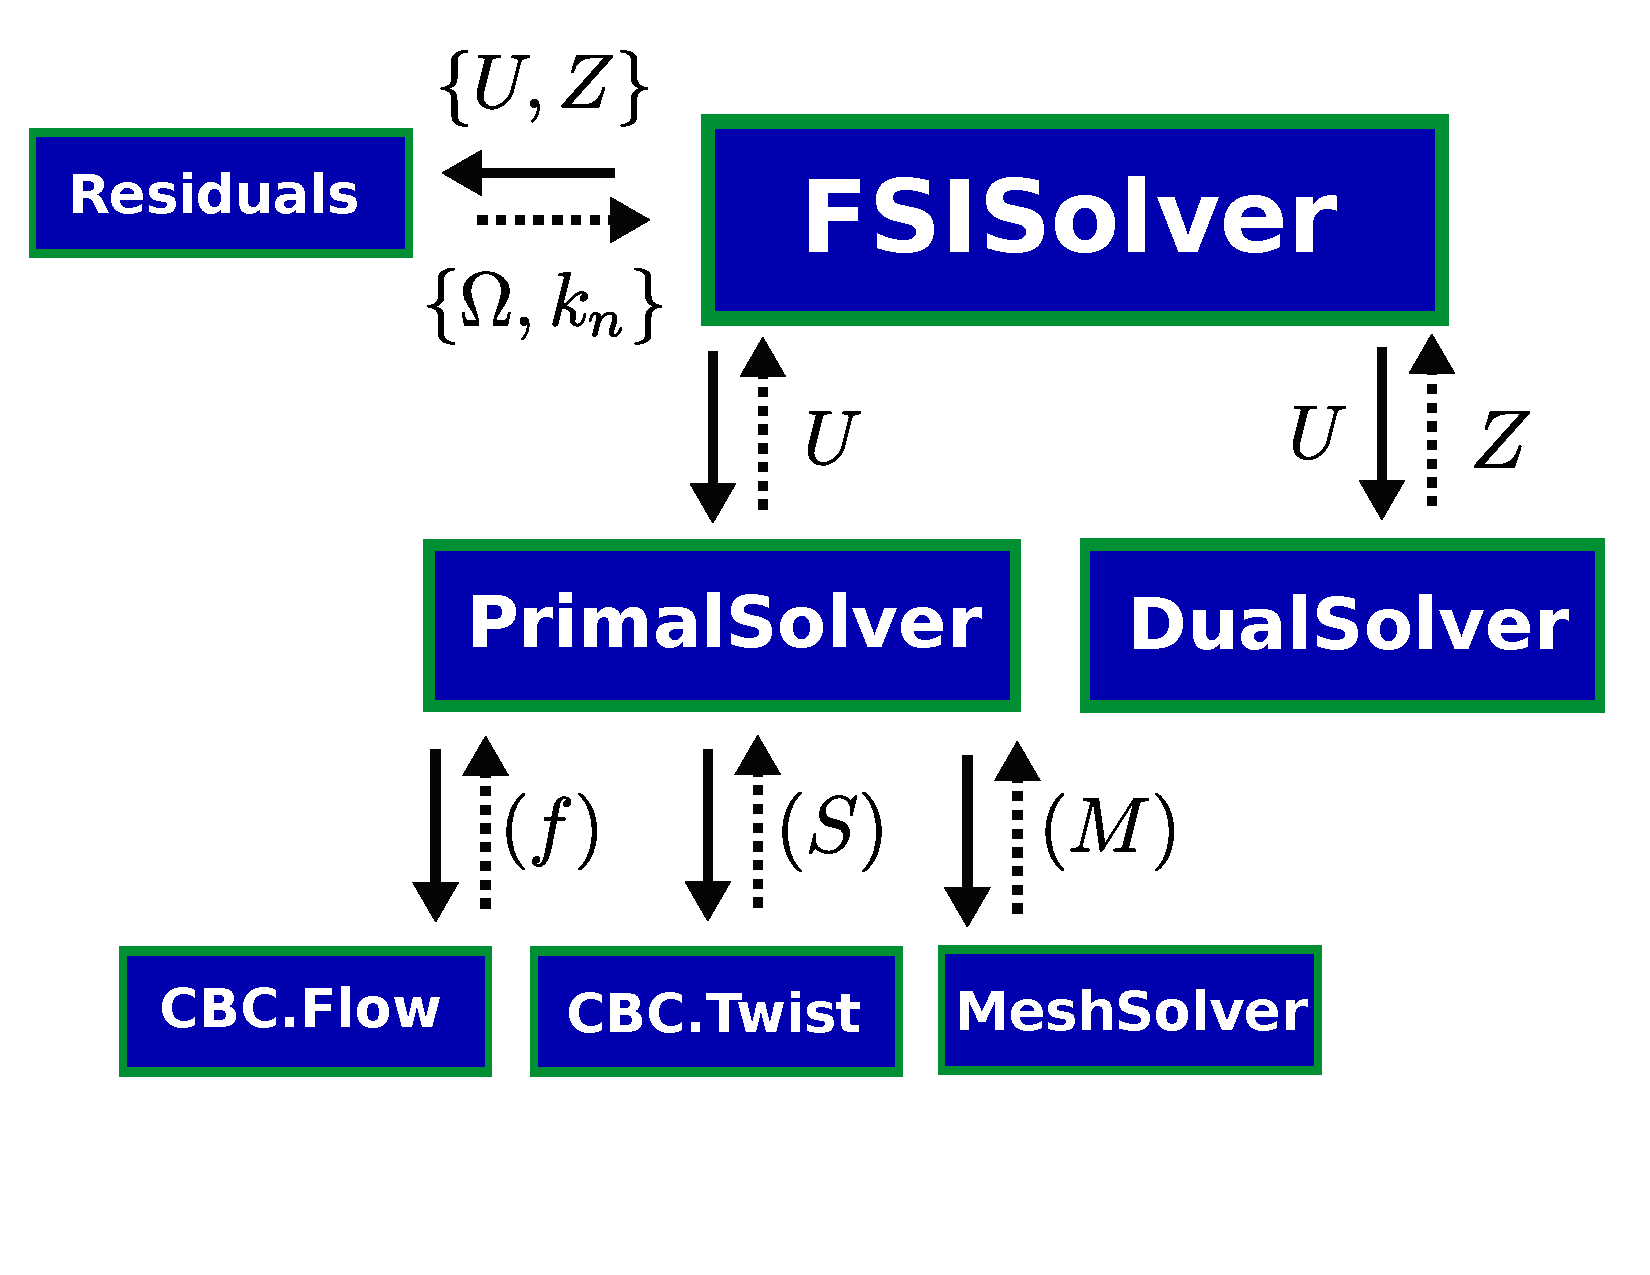
\includegraphics[width=1.0\textwidth]{chapters/selim/pdf/adaptive.pdf}
\caption{A schematic picture of the adaptive FSI algorithm. The primal
  problem ~\eqref{selim:eq:FSIsystem} is solved iteratively in the
  \texttt{PrimalSolver} and the solution $U$ is passed to the
  \texttt{FSISolver}. The dynamic time step $k_n$ is calculated for
  each time step in the iterative solver \texttt{PrimalSolver}
  using~\eqref{selim:eq:timestep2} in the module
  \texttt{Residuals}. After the primal problem is solved on the entire
  time interval, the dual problem is solved with the same time steps
  as in the primal solution in the module \texttt{DualSolver}. Once
  the dual is solved, the error estimates are evaluated and a new mesh
  is created.}
\end{figure}

\begin{figure}
\label{selim:fig:FSISolver}
\caption{The adaptive solver class \texttt{FSISolver}. Here, the
  problem specific data is passed as the variable \texttt{problem}. In
  the first adaptive loop, we make an initial guess of the stability
  factor $\mathcal{S}(T)=1$ in order to adapt the time step in the
  first loop.  The variable name \texttt{error} represents the sum of
  $E_h + E_k + E_c$ in~\eqref{selim:eq:aposteriori} and
  \texttt{indicator} represents $\eta_T$ in~\eqref{selim:eq:dorfler}.}
\begin{python}
class FSISolver(CBCSolver):

    def __init__(self, problem):
        "Initialize FSI solver"
            ...
    def solve(self):
        "Solve the FSI problem (main adaptive loop)"

        # Create empty solution (return value when primal is not solved)
        U = 5*(None,)

        # Initial guess for stability factor
        ST = 1.0

        # Adaptive loop
        while True:
            # Solve primal problem
            if self.parameters["solve_primal"]:
                primal_solver = PrimalSolver(self.problem, self.parameters)
                U = primal_solver.solve(ST)

            else:
                info("Not solving primal problem")

            # Solve dual problem
            if self.parameters["solve_dual"]:
                dual_solver = DualSolver(self.problem, self.parameters)
                dual_solver.solve()
            else:
                info("Not solving dual problem")

            # Estimate error and compute error indicators
            if self.parameters["estimate_error"]:
                error, indicators, E_h = estimate_error(self.problem)
            else:
                info("Not estimating error")
                error = 0

            # Check if error is small enough
            tolerance = self.parameters["tolerance"]
            if error <= tolerance:
                break
            else:

            # Check if mesh error is small enough
            mesh_tolerance = tolerance * self.problem.space_error_weight()
            if E_h <= mesh_tolerance:
                info("Freezing the current mesh")
            else:
                # Refine mesh
                problem = self.problem
                mesh = refine_mesh(problem,
                                   problem.mesh(),
                                   indicators)
                problem.init_meshes(mesh)

        # Return solution
        return U
\end{python}
\end{figure}


%------------------------------------------------------------------------------
\section{Numerical examples}

To demonstrate the above described adaptive algorithm, we solve two
simple 2D problems. These problems have different characteristics and
they demonstrate how the proposed adaptive algorithm provides both an
adequate adaptive mesh refinement and time step selection.

%------------------------------------------------------------------------------
\subsection{Channel with flap}

The first problem is a channel flow with a completely immersed
structure called ``the flap''. The computational domain is given by
$\Omega = (0, 1)\times (0,4)$, with the structure domain $\OS = (1.4,
1.6)\times (0, 0.5)$ and the fluid domain $\OF = (\Omega\setminus
\OS)^{\circ}$. For boundary conditions, we consider a pressure driven
flow and the flap is attached at the channel wall. As goal functional,
we have used the displacement of the structure in the positive
$x_1$-direction, that is,
\begin{equation}
\label{selim:eq:goalfunctional_channel}
\M_{_{S}}(v_{_{S}}) = \int_0^T \langle \psi^t_{_{S}},\;
v_{_{S}}\rangle \dt,
\end{equation}
where $\psi^t_{_{S}} = (1,0)$. The adaptive primal FSI solution is
depicted in Figure~\ref{selim:fig:primal_channel} and the
corresponding dual solutions are illustrated in
Figure~\ref{selim:fig:dual_channel_ZF}, Figure~\ref{selim:fig:dual_channel_ZS}
and in Figure~\ref{selim:fig:dual_channel_ZM}.
\begin{figure*}
  \label{selim:fig:primal_channel}
  \caption{The adaptive FSI solution to the channel with flap problem
    depicted in the current domain $\omega(t)$. Here, the fluid
    velocity solution is illustrated using streamlines.}
  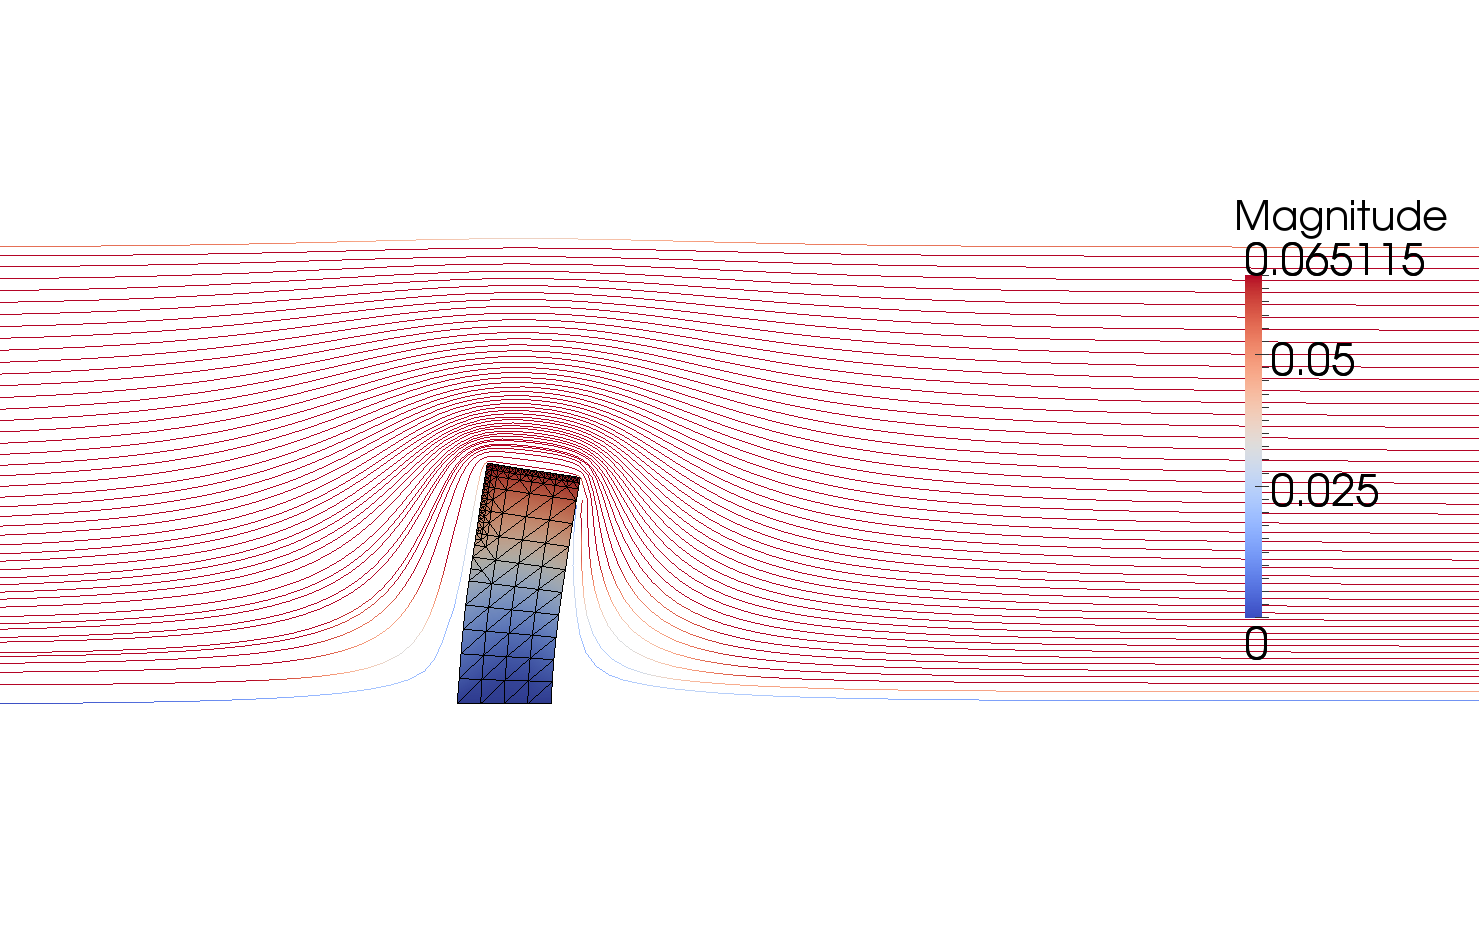
\includegraphics[width=1.0\textwidth]{chapters/selim/png/channel.png}
\end{figure*}

\begin{figure}
  \label{selim:fig:channel_zoom_mesh}
  \caption{A close view of the adaptive mesh. The mesh is refined in
    the immediate area around the structure. The problem is monotone
    in the sense that the structure bends until it reaches a fixed
    position. The physical constants related to this problem are:
    $(\rhoF,\mu_{_{F}}) = (1, 0.02)$ and $(\rho_{_{S}},\mu_{_{S}},
    \lambda_{_{S}}) = \tfrac{1}{4}(15, 75, 125)$.}
  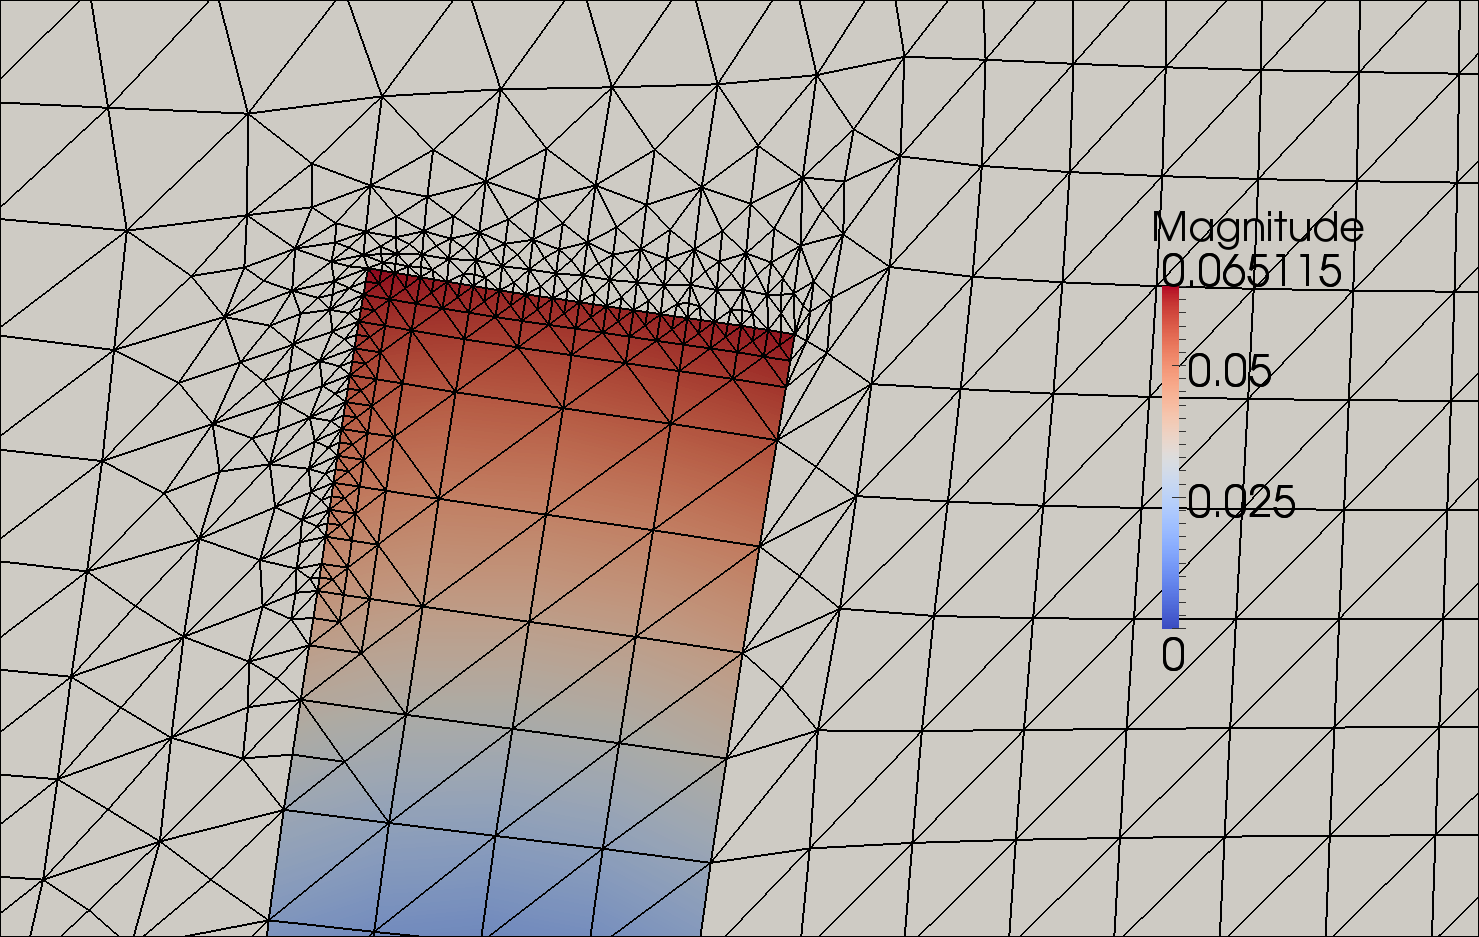
\includegraphics[width=0.95\textwidth]{chapters/selim/png/channel_test_zoom.png}
\end{figure}
\begin{figure}
  \label{selim:fig:dual_channel_ZF}
\caption{The dual fluid velocity solution  $Z_{_{F}}$  to the channel with flap problem solved in
  the reference domain $\Omega$. Since the only
  driving force of the fully coupled dual problem is the goal
  functional~\ref{selim:eq:goalfunctional_channel}, the dual fluid is
  concentrated around the top left corner of the structure where the
  structure displacement is large.}
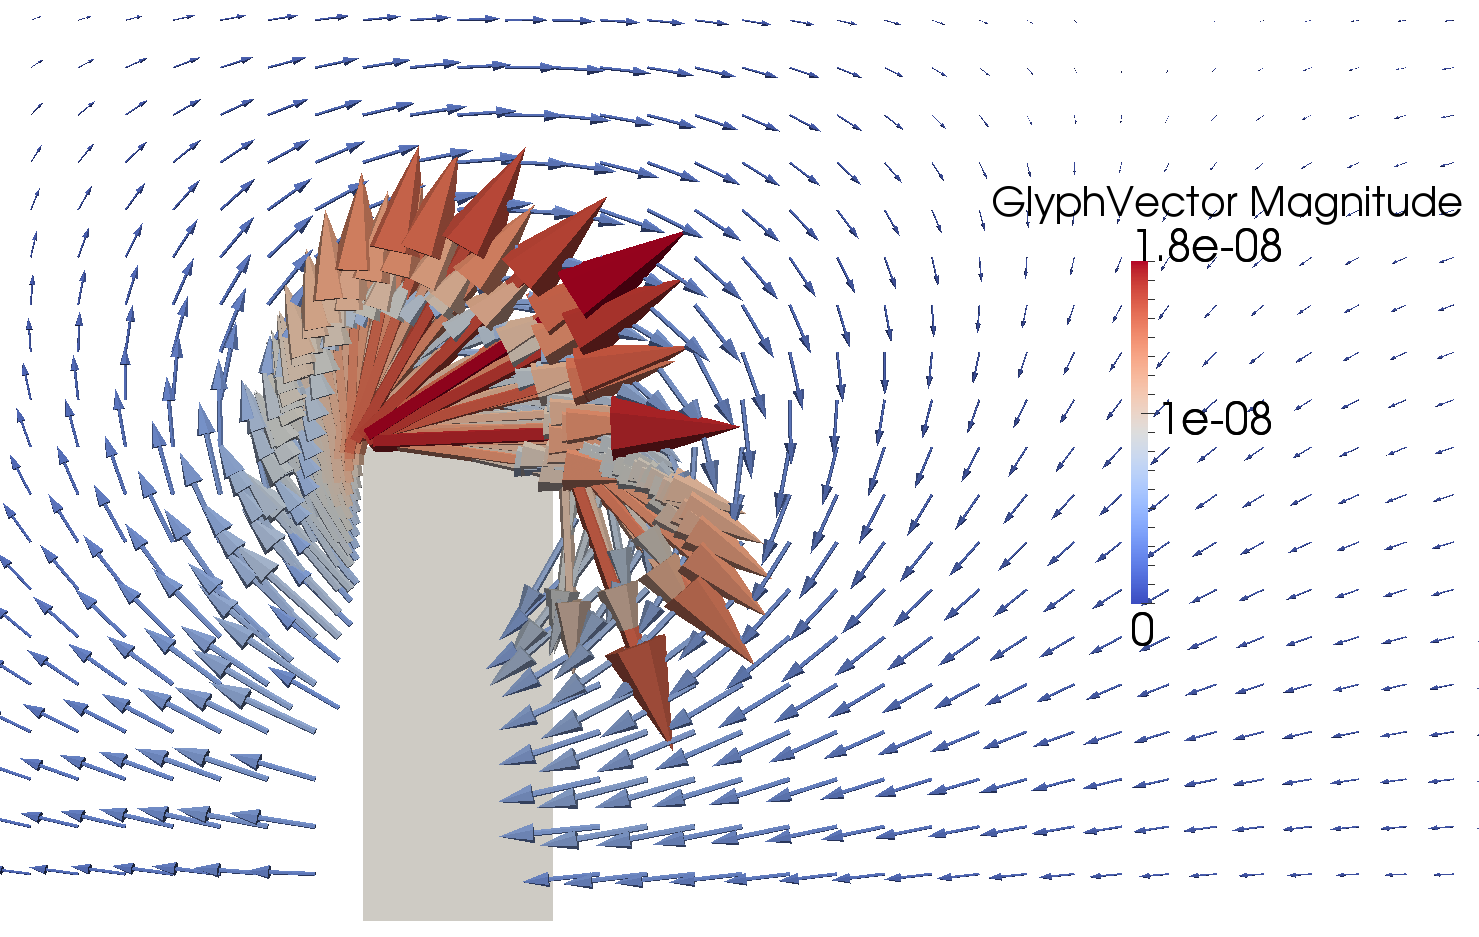
\includegraphics[width=1.0\textwidth]{chapters/selim/png/channelZF.png}
\end{figure}
\begin{figure}
  \label{selim:fig:dual_channel_ZS}
\caption{The dual structure solution $Z_{_{S}}$ to the channel with
  flap problem solved in the reference domain $\Omega$. The dual
  structure displacement $Z$ illustrates the choice of goal
  functional in~\eqref{selim:eq:goalfunctional_channel}.}
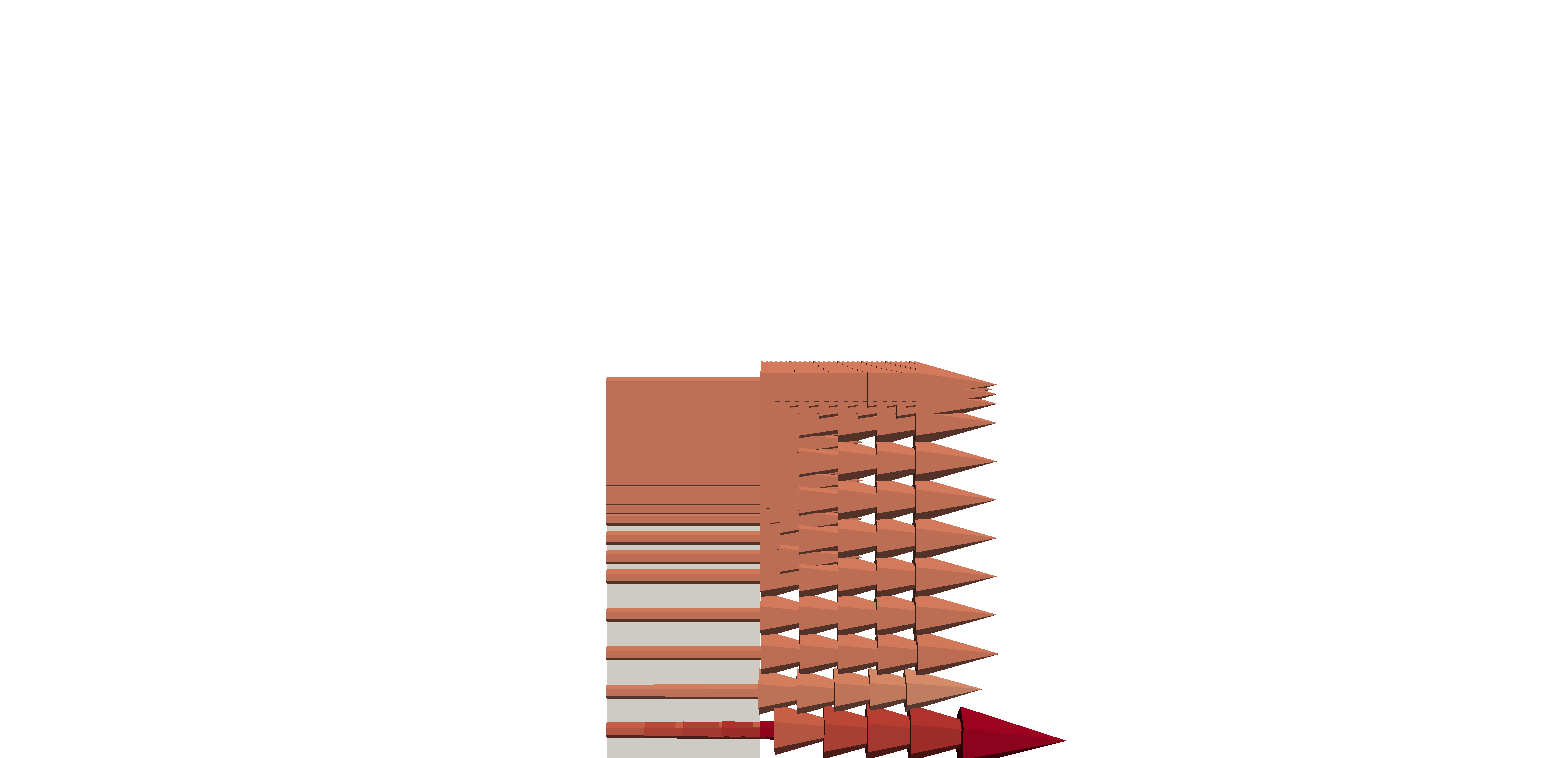
\includegraphics[width=1.0\textwidth]{chapters/selim/png/channelZS.png}
\end{figure}
\begin{figure}
  \label{selim:fig:dual_channel_ZM}
\caption{The dual mesh displacement $Z_{_{M}}$ to the channel with
  flap problem solved in the reference domain $\Omega$. The dual mesh
  displacement is large close to the the top right corner of the
  structure which is expected since the mesh in the current domain
  $\omega(t)$ is heavily compressed in this region.}
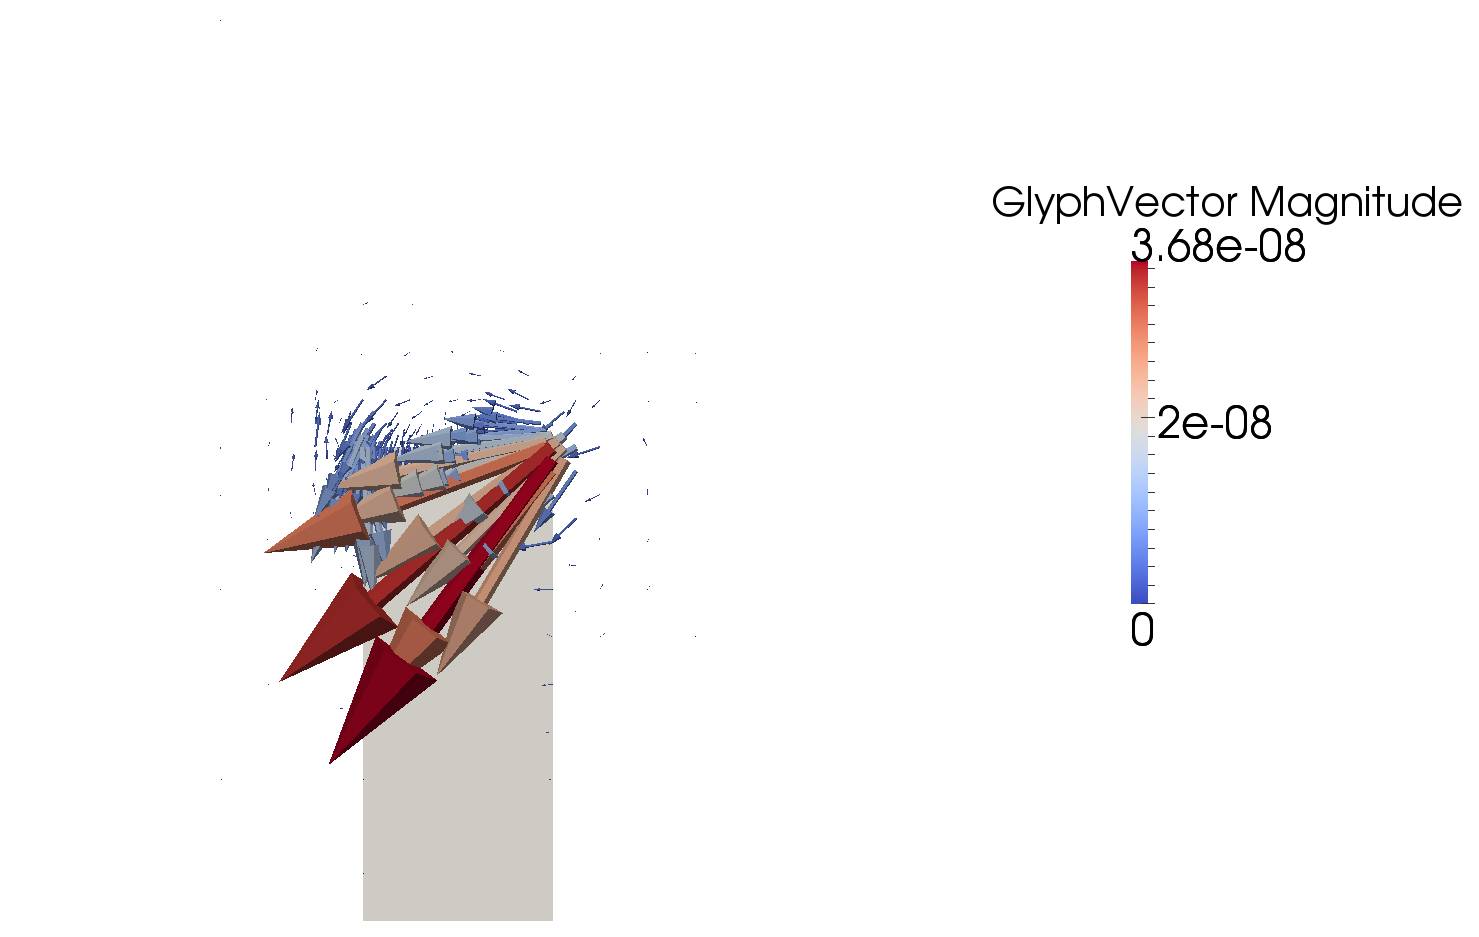
\includegraphics[width=1.0\textwidth]{chapters/selim/png/channelZM.png}
\end{figure}

%------------------------------------------------------------------------------
\subsection{Driven cavity with an elastic bottom}

The second problem is a driven cavity with an elastic bottom. Here,
the computational domain is given by $\Omega = (0,2)\times (0,2)$,
with structure domain $\OS = (0, 2)\times (0, 0.5)$ and the fluid
domain $\OF = (\Omega\setminus \OS)^{\circ}$. At the top of the fluid
domain, the fluid has the regularized tangential velocity profile
\begin{equation}
\uF =
\left\{
\begin{array}{lcl}
4x,& &x\in[0, 0.25],\\
1,& &x\in(0.25 ,1.75),\\
4(2-x),&  &x\in[1.75, 2],
\end{array}
\right.
\end{equation}
for all $t \in [0,5]$. The structure is attached at the bottom and the
goal functional is set as the structure displacement in the positive
$x_2$-direction, that is,
\begin{equation}
\label{selim:eq:goalfunctional_cavity}
\M_{_{S}}(v_{_{S}}) = \int_0^T \langle \psi^t_{_{S}},\; v_{_{S}}\rangle \dt,
\end{equation}
where $\psi^t_{_{S}}=(0,1)$. In contrast to the
previous problem, the solution, and in particular the structure
displacement, varies substantially over time. The adaptive primal FSI
solution is depicted in~Figure~\ref{selim:fig:primal_cavity} and the
dynamic time step size is illustrated
in~Figure~\ref{selim:fig:cavity_timestep}.
\begin{figure}
\label{selim:fig:primal_cavity}
\caption{The adaptive solution to the driven cavity problem with an
  elastic bottom at time $t=2$. The structure does not reach a steady
  position; instead the structure moves up and down at the common
  fluid--structure boundary. In this problem, the physical parameters
  are given by $(\rhoF,\mu_{_{F}}) = (1, 1)$ and
  $(\rho_{_{S}},\mu_{_{S}}, \lambda_{_{S}}) = (1, 3, 3)$. In the
  bottom figure a close up view of the refined mesh at the FSI boundary is
  given.}
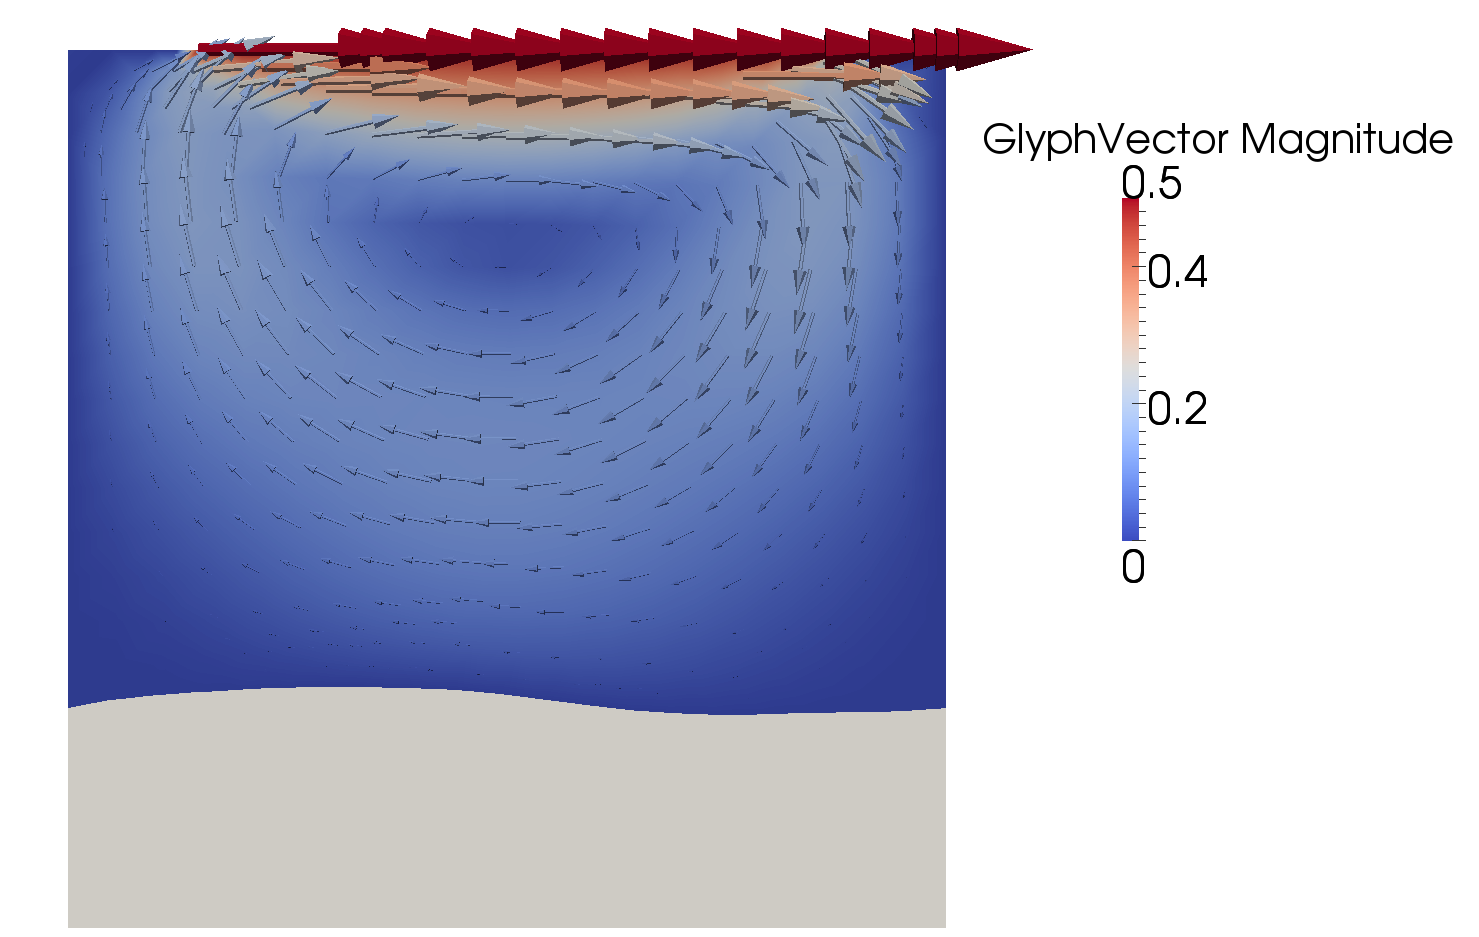
\includegraphics[width=0.9\textwidth]{chapters/selim/png/cavity_large.png}

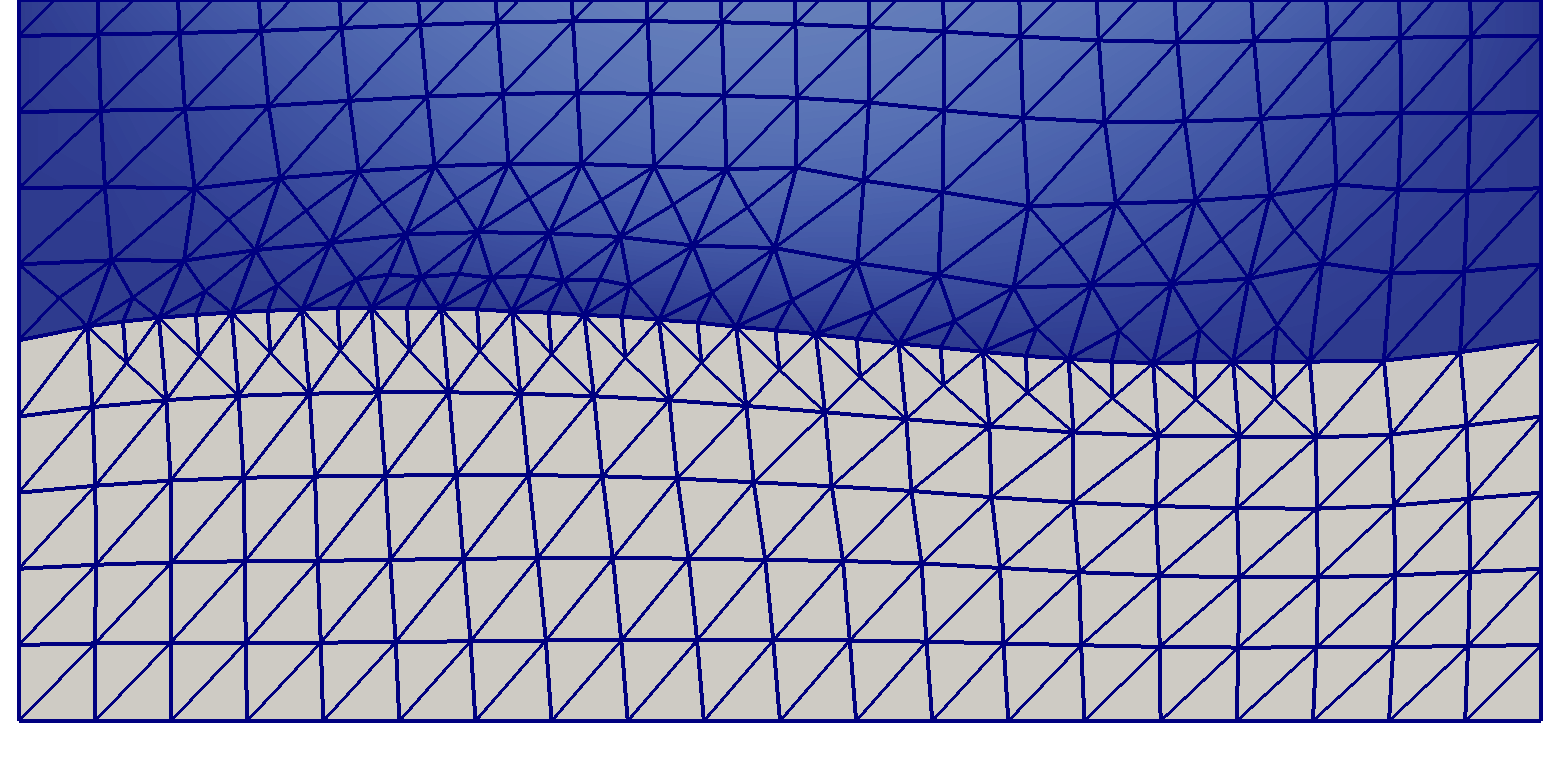
\includegraphics[width=0.95\textwidth]{chapters/selim/png/zoom_cavity.png}
\end{figure}
 \begin{figure}
\label{selim:fig:cavity_timestep}
\caption{The time step $k_n$ and the algebraic residual $r_k^n$ as
  a function of time. As seen in the picture, the solution has a large
  variation in terms of the magnitude of the residual $r_k^n$.}
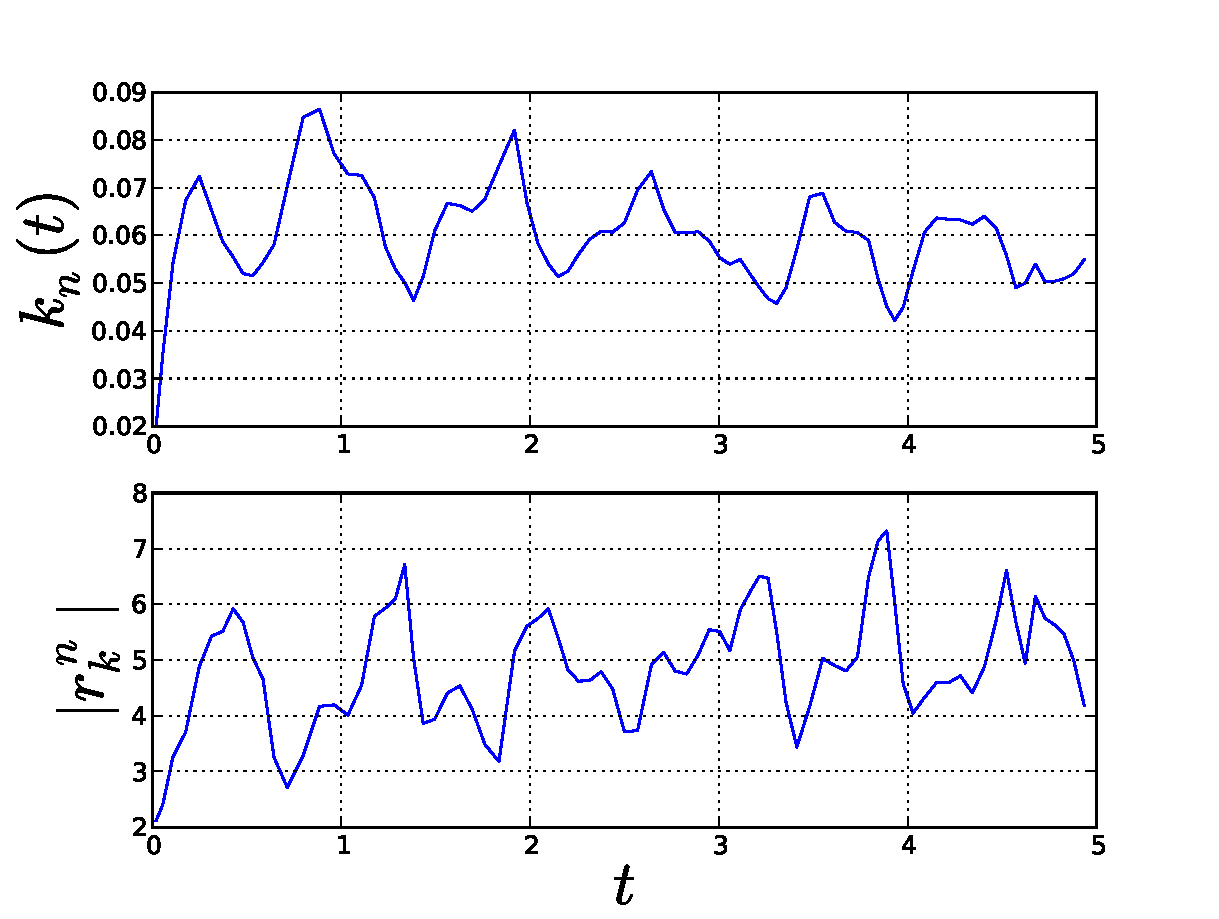
\includegraphics[width=0.9\textwidth]{chapters/selim/pdf/plot.pdf}
\end{figure}

%------------------------------------------------------------------------------
\section{Conclusions}

In this chapter, an adaptive finite element method for FSI problems
has been formulated and its implementation in FEniCS has been
demonstrated. By relating the fully coupled partitioned FSI
problem~\eqref{selim:eq:FSIsystem} in a moving domain to a dual
problem~\eqref{selim:eq:dual} posed on a fixed reference domain, an
adapted space and time discretization is obtained.



% Local Variables:
% mode: latex
% mode: flyspell
% mode: auto-fill
% End:

